\documentclass[11pt]{article}
\usepackage[final]{acl}
\usepackage{times}
\usepackage{latexsym}
\usepackage[T1]{fontenc}
\usepackage[utf8]{inputenc}
\usepackage{microtype}
\usepackage{inconsolata}
\usepackage{graphicx}
\usepackage{booktabs}
\usepackage{amsmath}
\usepackage{multirow}
\usepackage{tikz}
\usetikzlibrary{positioning,arrows.meta,fit}

\title{Judge-Guided Generation, Selection and Repair of Inline Non-Verbal Sounds in Vietnamese Speech Synthesis}

\author{Hieu Ngo \quad Thuan Nguyen \quad Huy Nguyen \\
  Trivita AI \\
  \texttt{\{hieu.ngo, thuan.nguyen, huy.nguyen\}@trivita.ai}}

\begin{document}
\maketitle

\begin{abstract}
We describe the WiTake system for the VLSP 2026 ViNV-TTS shared task: Vietnamese text-to-speech in which inline tags
(\texttt{[laughter]}, \texttt{[breathing]}, \texttt{[sniff]}, \texttt{[throatclearing]}) must be realised as the
corresponding sound at the tagged position, both for speakers seen in training (Track~A) and for zero-shot cloning from a
reference clip (Track~B). The system starts from the open masked non-autoregressive TTS model OmniVoice and adds
(i)~supervised fine-tuning on the official data plus synthetic rare-class events, (ii)~a class-aware preference
optimisation (DPO) stage adapted to masked generative TTS, (iii)~\emph{tag-contrastive} classifier-free guidance that
contrasts the tagged text with the same text without tags, (iv)~best-of-16 selection over two engines with automatic
judges weighted like our proxy of the official score, (v)~splicing of real non-verbal clips where the judges still find a tag
missing, and (vi)~a loudness-levelling step that maps generated non-verbal events onto the level distribution of real
recordings. On the public test set, tag-contrastive guidance alone raises the hit rate of a held-out tag-ASR judge
from .58 to .83 (Track~A, single draw). The full system reaches .93/.96 (Track~A/B) on that judge, which is optimistic
because the judge also drives selection, and about .89 on an independent audit judge, with automatic WER of
1.5/1.7\% and unchanged naturalness proxies. The system is packaged as an offline single-GPU Docker image. We also
report the many things that did not help.
\end{abstract}

\section{Introduction}

Conversational speech is full of non-verbal vocalisations (NVs): laughter, audible breaths, sniffs, throat clearing.
Modern zero-shot TTS models reproduce the timbre and prosody of a prompt well but rarely produce such events on demand,
and when an NV tag is given in the text the model often ignores it or reads it as noise. The ViNV-TTS task asks for
Vietnamese speech in which four NV classes are produced exactly where an inline tag places them.

Three properties of the task shaped our system. First, the classes are very unbalanced: the official training set has
3{,}733 breathing tags but only 117 sniff and 115 throat-clearing tags (Table~\ref{tab:data}). Second, NV placement accuracy
is the largest single term of the official score (weight .3, against .1--.2 for every other term), so a missed tag
costs more than a small loss in naturalness. Third, NV realisation is cheap to \emph{check} automatically
(an aligned word gap can be classified) but hard to \emph{guarantee} in one sampling pass. We therefore treat generation
as a generate--judge--repair loop: make the model more likely to produce the event (fine-tuning, DPO, guidance), sample
several candidates and pick the best with judges, and repair what is still missing.

Our contributions are: a tag-contrastive guidance term for masked generative TTS that raised the held-out tag hit rate
from .58 to .83 at no training cost; a class-aware DPO recipe for masked non-autoregressive TTS; a selection-and-splice
pipeline whose gains we verify with judges that were never used for selection; an NV loudness-levelling step that
corrects the over-loud events that every detectability-driven component produces; and an honest list of negative
results.

\section{Task and Data}

\paragraph{Task.} Each test item gives a target text with inline tags and a reference (prompt) clip with its transcript.
Track~A uses speakers from the training set, Track~B unseen speakers. The official score\footnote{\url{https://vlsp.org.vn/vlsp2026/eval/vinvtts}}
combines NV placement accuracy (NVPA), human-rated naturalness (SN) and quality (Q), a human SUS-test WER, an automatic
WER (aWER, Zipformer) and speaker similarity (SS, ECAPA-TDNN): Track~A $= .3\,\mathrm{NVPA} + .2\,\mathrm{SN} +
.2\,\mathrm{Q} + .1(1{-}\mathrm{WER}) + .1(1{-}\mathrm{aWER}) + .1\,\mathrm{SS}$, and Track~B $= .3\,\mathrm{NVPA} +
.15\,\mathrm{SN} + .15\,\mathrm{Q} + .1(1{-}\mathrm{WER}) + .1(1{-}\mathrm{aWER}) + .2\,\mathrm{SS}$.

\paragraph{Automatic proxy.} During development we optimised an automatic proxy with four terms and the weights we
used throughout development (Track~A: NV .3, WER .15, MOS .15, SS .1; Track~B: NV .3, WER .1, MOS .1, SS .2),
normalised by their sum:
\begin{align*}
\textit{off}_T = \tfrac{1}{0.7}\big(&.3\,\mathrm{NV} + w^T_{\mathrm{wer}}(1{-}\mathrm{WER}) \\
&+ w^T_{\mathrm{mos}}\tfrac{\mathrm{pMOS}}{5} + w^T_{\mathrm{ss}}\,\mathrm{SS}\big)
\end{align*}
with WER from a Vietnamese Zipformer transducer \citep{yao2024zipformer,zipformervi}, pMOS = DNSMOS OVRL
\citep{reddy2022dnsmos}, SS = ECAPA-TDNN cosine similarity to the prompt \citep{desplanques2020ecapa,ravanelli2021speechbrain}, and NV = hit rate
of our tag-ASR judge v3 (Section~\ref{sec:judges}). We write \textit{offA}/\textit{offB} for Track~A/B. Human-rated
terms are not included.

\paragraph{Data.} We used the official training and development sets (Table~\ref{tab:data}), VocalSound
\citep{gong2022vocalsound} as a source of sniff and throat-clearing events, and, as text only, sentences transcribed from
public Vietnamese football talk videos for preference-optimisation prompts. The public test set has 210 Track~A items
(7 speakers) and 120 Track~B items (4 unseen speakers); with 32--56 tags per class, differences of about .03 in a
per-class hit rate are within noise. For model selection we also held out 114 training utterances (\emph{evalR}).

\begin{table}[t]
\centering\small
\resizebox{\columnwidth}{!}{\begin{tabular}{lrrrrrr}
\toprule
split & utts & spk & hours & breath & laugh & sniff / throat \\
\midrule
train & 1739 & 189 & 5.90 & 3733 & 681 & 117 / 115 \\
dev   &  316 &  46 & 1.04 &  674 & 102 &  14 / 19 \\
\bottomrule
\end{tabular}}
\caption{Official ViNV-TTS data (tag counts per class).}
\label{tab:data}
\end{table}

\section{System}

Figure~\ref{fig:pipeline} shows the pipeline. Two fine-tuned OmniVoice engines generate 8 candidates each; every
candidate is scored by automatic judges; the best one under the proxy-weighted utility is kept; missing events are
spliced in from real recordings; and NV loudness is levelled.

\begin{figure}[t]
\centering
\resizebox{\columnwidth}{!}{%
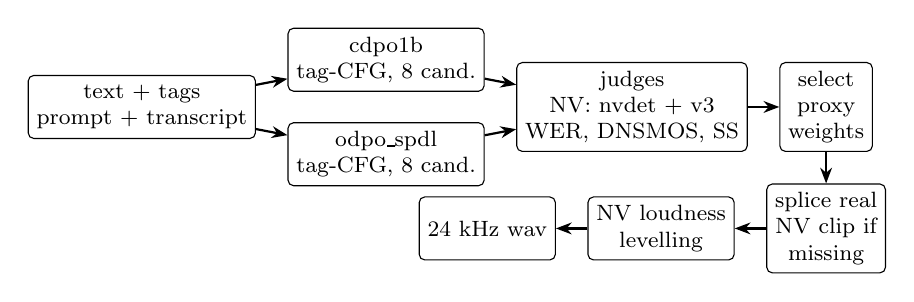
\begin{tikzpicture}[node distance=4mm and 4mm, font=\footnotesize,
  box/.style={draw, rounded corners=2pt, align=center, minimum height=8mm, inner sep=3pt},
  arr/.style={-{Stealth[length=2mm]}, thick}]
\node[box] (in) {text + tags\\prompt + transcript};
\node[box, right=of in, yshift=6mm] (e1) {cdpo1b\\tag-CFG, 8 cand.};
\node[box, right=of in, yshift=-6mm] (e2) {odpo\_spdl\\tag-CFG, 8 cand.};
\node[box, right=of e1, yshift=-6mm] (j) {judges\\NV: nvdet + v3\\WER, DNSMOS, SS};
\node[box, right=of j] (s) {select\\proxy\\weights};
\node[box, below=of s] (sp) {splice real\\NV clip if\\missing};
\node[box, left=of sp] (lv) {NV loudness\\levelling};
\node[box, left=of lv] (out) {24 kHz wav};
\draw[arr] (in) -- (e1); \draw[arr] (in) -- (e2);
\draw[arr] (e1) -- (j); \draw[arr] (e2) -- (j);
\draw[arr] (j) -- (s); \draw[arr] (s) -- (sp); \draw[arr] (sp) -- (lv); \draw[arr] (lv) -- (out);
\end{tikzpicture}}
\caption{Inference pipeline (v5). In our public-test runs, Track~A additionally re-generates (``inpaints'') missed tags inside the
primary engine before selection; the submitted image runs every item with the Track~B settings.}
\label{fig:pipeline}
\end{figure}

\subsection{Base model}
OmniVoice \citep{omnivoice} is a masked generative (non-autoregressive) TTS model, like MaskGCT
\citep{wang2024maskgct}: a transformer predicts the masked audio tokens of a multi-codebook codec (the Higgs Audio~2
tokenizer) conditioned on text, the prompt transcript and the prompt's audio tokens, and fills the sequence in 32
iterative steps with classifier-free guidance. Its zero-shot cloning was clearly stronger than the alternatives we tried
(Section~\ref{sec:negative}). Out of the box it ignores NV tags.

\subsection{Supervised fine-tuning with synthetic rare events}
We fine-tune OmniVoice with LoRA \citep{hu2022lora} using the official recipe on the training set, with the tags kept
as text and rare classes oversampled (square-root sampling). Because sniff and throat clearing have only about 115
examples each, we generate synthetic examples: VocalSound events are converted to the voice of a training speaker with
Seed-VC \citep{seedvc} and inserted into that speaker's utterances at a word gap, then filtered with our rare-class
judge. We also add laughter clips generated by an earlier fine-tuned TTS model and filtered with the laughter judge and
WER $\le$ .10. The resulting model (\emph{omft\_tdl4000}, 4{,}000 steps) uses the synthetic throat-clearing clips but no
synthetic sniffs; it is the parent of both served engines. Its original synthetic throat clips were not kept, so the
released set (277 clips: 174 throat clearing, 103 sniff) is a regenerated one. Continuing fine-tuning from
omft\_tdl4000 on the official data alone, without the synthetic and laughter clips, cut throat recall on evalR from .69
to .28.

\subsection{Class-aware DPO for masked generative TTS}
\label{sec:dpo}
Fine-tuning made the model capable of the events but did not make it reliable on rare classes. We therefore applied
on-policy preference optimisation \citep{rafailov2023dpo}. Masked generative models have no tractable sequence
likelihood, so we use the masked cross-entropy as a likelihood surrogate: for a target token sequence $y$, $\ell(y)$ is
the codebook-weighted mean cross-entropy on masked positions, averaged over $K{=}4$ stratified mask ratios, with the
policy and the frozen reference sharing every mask. The loss is
\begin{align*}
\mathcal{L} = &-\log\sigma\big(\beta[(\ell_{\mathrm{ref}}(y_w){-}\ell_\theta(y_w)) \\
&- (\ell_{\mathrm{ref}}(y_l){-}\ell_\theta(y_l))]\big) + \gamma\,\ell_\theta(y_w)
\end{align*}
where the last term anchors the policy to the chosen sample.

\paragraph{Pairs.} We built 1{,}921 prompts (1{,}660 football-talk sentences with one or two inserted tags, 15\% of
them sentence-initial and 15\% sentence-final; 261 single-class training texts), each with a 3--9\,s reference clip of a
training speaker. No public-test text or audio was used. The SFT model generated 8 candidates per prompt (15{,}368 in
total). Each tag was judged by the AST-based detector and a class-specific judge (Section~\ref{sec:judges}). The chosen
sample realises every tag with WER $\le$ .15 and SS above the prompt median minus .05; the rejected sample is a candidate
of the same prompt in which the target-class tag is missing. We kept at most one pair per prompt and balanced the classes
(649 pairs: breathing 179, throat 179, laughter 153, sniff 138), then trained for 1{,}298 single-pair steps (twice the pair count, pairs sampled with replacement,
gradient accumulation 8,
$\beta{=}5$, lr $5\cdot10^{-5}$, LoRA rank 16) and merged the adapter (\emph{cdpo1b}). The tag-ASR judge v3 was never
used to build pairs, so it remains a held-out judge for this step.

The second engine, \emph{odpo\_spdl}, comes from a separate SFT run that also uses the synthetic sniff clips followed by DPO on 600
training prompts $\times$ 4 on-policy candidates, ranked by an earlier Whisper-based tag-ASR \citep{radford2023whisper}
and the AST detector.

\subsection{Tag-contrastive guidance (tag-CFG)}
Standard classifier-free guidance \citep{ho2022cfg} contrasts the conditional logits $c$ with unconditional ones $u$.
We add a second contrast against the logits $c_{\setminus\mathrm{tag}}$ obtained with the same text \emph{with the tags
removed}:
\begin{equation*}
\log p = c + g\,(c-u) + w\,(c - c_{\setminus\mathrm{tag}}).
\end{equation*}
The extra term amplifies exactly what the tags change in the prediction, i.e.\ the NV events. All three rows are
computed in one batched forward pass per decoding step. We use $g{=}2, w{=}3$ for Track~A and $g{=}6, w{=}5$ for
Track~B on the primary engine, chosen on a partial grid over $g\in\{2,4,6\}$ and $w\in\{0,3,5,7\}$ run on the SFT parent.

\subsection{Verify-and-inpaint (Track~A)}
For Track~A the primary engine checks each candidate after decoding: Zipformer word timestamps locate the gap of every
tag, the AST detector classifies it, and for every missed tag the audio tokens of that gap ($\pm$0.12\,s plus a few
inserted frames) are re-masked and regenerated with all other tokens fixed, for up to $k{=}2$ rounds. Inpainting all 8
candidates gives the selector more tag-complete candidates. Repairing only the selected candidate kept almost none of
the gain (+.002 vs +.020 NV measured by nvdet, which also decides what to inpaint).

\subsection{Judges and selection}
\label{sec:judges}
\begin{itemize}\itemsep0pt
\item \textbf{nvdet}: AST \citep{gong2021ast} embeddings of the aligned tag gap with a logistic-regression head over
\{none, 4 classes\}, trained on events cut from the official training set.
\item \textbf{tag-ASR v3}: Qwen3-ASR-1.7B \citep{qwen3asr} fine-tuned to transcribe the training set \emph{with} inline
tags. A tag counts as realised when the transcript contains it at the right position. Dev precision/recall: breathing
.90/.89, laughter .72/.82, but sniff .36/.29 and throat .60/.32.
\item \textbf{Class judges}: LaughterSegmentation \citep{laughterseg} for laughter, and frame-level PretrainedSED models
\citep{schmid2024psed} (BEATs, ATST-F, M2D) with small logistic heads for sniff and throat clearing.
\item \textbf{Audit judge} (evaluation only): CLAP \citep{wu2023clap} + WavLM \citep{chen2022wavlm} features with a
logistic head. It shares no model with the other judges and was never used by generation, selection or splicing.
\end{itemize}
Each of the 16 candidates gets the proxy-weighted utility \textit{off}$_T$ with NV $=$ mean over tags of
$\tfrac12$(nvdet $p_{\mathrm{tag}}$ + v3 hit). In a leave-one-judge-out study, nvdet alone as the selector overfitted as
$N$ grew (held-out v3 NV on Track~B .83$\rightarrow$.79 from $N{=}8$ to 24), while the nvdet+v3 average was the most
stable rule (held-out class-judge NV .91--.98).

\subsection{Splicing real NV clips}
If, on the selected candidate, the tag-ASR or the class judge still finds a tag missing (decision rule \emph{any}),
the tag's word gap is replaced by 80\,ms pause + a real NV clip + 120\,ms pause with 15\,ms cross-fades. Clips come from
a bank of events cut from the official training set (breathing 1{,}021, laughter 337, sniff 65, throat 80), filtered by
nvdet confidence, SNR and length. For Track~A the clip comes from the same speaker when available; for Track~B from the
three ECAPA-nearest bank speakers. Converting bank clips to the prompt voice with Seed-VC removed the NV character
(nvdet hit rate .83$\rightarrow$.31) for +.002 SS, so we splice unconverted clips.

\subsection{NV loudness levelling}
Tag-CFG, judge-ranked DPO, best-of-$N$ and splicing all reward \emph{detectable} events. Measured relative to the
surrounding speech, our laughter and throat clearing sat about 3--4\,dB and our sniffs 9--12\,dB louder than in
real recordings. For each class
we map the system's NV-to-speech level distribution onto the distribution measured on the training set with a 1-D
quantile (optimal-transport) map, and only ever attenuate the aligned NV span, with raised-cosine ramps (throat clearing
is moved only 60\% of the way, $\alpha{=}.6$; breathing is untouched). On the submitted outputs this reduced the
Wasserstein-1 distance between system and real NV levels from 5.9 to 3.6\,dB on Track~A and from 9.0 to 5.6\,dB on
Track~B, with WER, pMOS and SS unchanged.

\subsection{Deployment}
The organisers ran each image offline on one 40\,GB GPU with a 60-minute limit for about 50 items. Our image
contains all weights and four Python environments; per-process GPU memory caps keep the five services below 35\,GB
(peak 34\,GB), and
the per-candidate count steps down (8$\rightarrow$4$\rightarrow$2$\rightarrow$1 per engine) if the measured speed
projects past the time budget. Every generation call is seeded from its text, so reruns are equivalent (GPU kernels are not
bit-exact). The image runs every item with the Track~B settings (reference-prompt cloning, Track~B guidance and
weights, ECAPA-nearest splice clips); verify-and-inpaint and same-speaker clips were used only in our public-test runs.
On one H100 a 50-item test takes 7.6\,min including 20\,s of start-up.

\section{Results}

\paragraph{Tag-CFG and inpainting.} Table~\ref{tab:cfg} isolates the guidance term on the SFT model (single draw, no
selection). Tag-CFG lifts the held-out v3 hit rate from .580 to .826 at $w{=}3$ and .897 at $w{=}5$, with unchanged WER
and SS and a small pMOS cost; inpainting adds a further gain on top.

\begin{table}[t]
\centering\small
\resizebox{\columnwidth}{!}{\begin{tabular}{lcccccc}
\toprule
config & NV & sniff & throat & WER & pMOS & SS \\
\midrule
plain ($w{=}0$) & .580 & .32 & .59 & .027 & 3.28 & .731 \\
$w{=}1$ & .759 & .52 & .77 & .026 & 3.27 & .732 \\
$w{=}3$ & .826 & .59 & .80 & .025 & 3.24 & .729 \\
$w{=}5$ & .897 & .71 & .95 & .029 & 3.21 & .734 \\
inpaint $k{=}3$ only & .750 & .50 & .86 & .027 & 3.28 & .731 \\
$w{=}3$ + inpaint $k{=}2$ & .884 & .66 & .96 & .026 & 3.25 & .732 \\
\bottomrule
\end{tabular}}
\caption{Tag-CFG and inpainting on public Track~A (SFT model, single draw, NV = tag-ASR v3 macro hit rate).}
\label{tab:cfg}
\end{table}

\paragraph{Splicing.} Table~\ref{tab:splice} shows splicing on the plain SFT outputs. Every decision rule improves every
independent judge, so the gain is not an artefact of deciding with the same judge that scores. Deciding with v3
(alone or with the class judges, \emph{any}) gives the highest NV and offA/offB in the table, but those rows are scored
by the judge that made the decisions; on nvdet, the judge independent of them, deciding with nvdet scores higher
(Track~A .772 vs .743 for \emph{any}). Adding nvdet's flags on top of \emph{any} lowers NV and the proxy on both
tracks, because replacing an event that was already right is a chance to do worse. In the full pipeline, with tag-CFG,
splicing becomes a safety net that fires on 3\% of tags (1\% in the submitted v5 run).

\begin{table}[t]
\centering\small
\resizebox{\columnwidth}{!}{\begin{tabular}{lcccc}
\toprule
decide & A: NV & A: offA & B: NV & B: offB \\
\midrule
no splice & .594 & .708 & .633 & .724 \\
nvdet & .754 & .775 & .750 & .775 \\
v3 & .817 & .801 & .828 & .813 \\
any (v3 or class judge) & .799 & .793 & .828 & .813 \\
any + nvdet & .781 & .786 & .781 & .794 \\
\bottomrule
\end{tabular}}
\caption{NV splicing on plain SFT outputs (public test). NV = tag-ASR v3 hit rate; in the v3 and
\emph{any} rows v3 also decided which tags to splice.}
\label{tab:splice}
\end{table}

\paragraph{DPO.} Under the full production recipe, cdpo1b improved over its SFT parent on both tracks (offA
.878$\rightarrow$.882, offB .870$\rightarrow$.875), mostly through sniff (Track~B .81$\rightarrow$.94) and
sentence-final tags on Track~B (.79$\rightarrow$.96). On evalR, sniff rose from .56 to .74 and throat from .84 to .88.
These differences are only one or two tags per class, so we treat them as consistent but small.

\paragraph{System evolution.} Table~\ref{tab:evolution} tracks the served system on the public test set. The largest
single gain comes from tag-CFG; the second engine, DPO and inpainting move the v3-scored numbers by at most .02 in
either direction. The audit judge (never used for selection) confirms the overall gain: its macro hit rate excluding
sentence-initial tags rose from .82 (plain) to .94--.95 (v2--v4) on both tracks, but between v2 and v4 its differences
are within noise. Levelling (v5) attenuates the over-loud events. This costs automatic NV (audit judge .94$\rightarrow$
about .89 on both tracks, v3 on Track~A .982$\rightarrow$.933), because the detectors hear quieter events less often,
but it is aimed at the human-rated naturalness that the proxy does not measure.

\begin{table}[t]
\centering\small
\setlength{\tabcolsep}{4pt}
\resizebox{\columnwidth}{!}{\begin{tabular}{lcccc}
\toprule
system & A: NV & offA & B: NV & offB \\
\midrule
SFT, best-of-8, plain gen.\ + splice & .897 & .845 & .898 & .849 \\
+ tag-CFG $w{=}3$ & .969 & .878 & .938 & .870 \\
v2: + 2nd engine, nvdet+v3 selector & .946 & .868 & .953 & .877 \\
v3: DPO engine (cdpo1b) & .969 & .879 & .945 & .874 \\
v4: + Track~A inpaint $k{=}2$ & .982 & .883 & .945 & .874 \\
v5: + NV levelling (submitted) & .933 & .863 & .961 & .879 \\
\midrule
WER / pMOS / SS (v5) & \multicolumn{2}{c}{.015 / 3.34 / .764} & \multicolumn{2}{c}{.017 / 3.33 / .812} \\
\bottomrule
\end{tabular}}
\caption{Served system on the public test (210 A / 120 B items). In every row v3 also drives selection and splicing, so its NV is
optimistic; each run is a single draw (NV noise about $\pm$.03).}
\label{tab:evolution}
\end{table}

\paragraph{Official evaluation.} Official results on the hidden test set were not available at the time of
writing.

\section{What Did Not Help}
\label{sec:negative}
\begin{itemize}\itemsep0pt
\item \textbf{Another base model.} A LoRA-tuned VoxCPM2\footnote{\url{https://huggingface.co/openbmb/VoxCPM2}} almost never produced mid-sentence NVs (hit rate $\approx$.03) and
was only +.01 SS over OmniVoice.
\item \textbf{More in-domain data.} We collected 62\,h of Vietnamese football and talk-show audio, labelled by our
tag-ASR and filtered by detectors. Every dose of it in continued fine-tuning lowered the public scores (NV .594$\rightarrow$.41--.46,
offA .708$\rightarrow$.63--.66); the automatic labels contained no usable sniff or throat clearing, and breathing dominated.
\item \textbf{Edge-position fine-tuning.} Oversampling clips cut so that events sit at the sentence edge raised
sentence-final sniff but collapsed throat clearing (public .52$\rightarrow$.20--.25), because the synthetic throat data
could not be replayed.
\item \textbf{Further DPO rounds.} Rounds 2 and 3 (more prompts, pMOS tie-breaks, multi-objective pairs) gained up to
+.012 offB but lost Track~A or the audit judge; the gains on judges seen during pair building did not transfer.
\item \textbf{Clean-label fine-tuning.} Removing 1{,}007 tags that all judges reject raised the audit judge (+.04--.08)
but lowered offA/offB by .002--.019.
\item \textbf{More candidates.} $N{=}24$ instead of 16 changed offA by $-.005$, within noise, at 2.4$\times$ the cost; on
Track~B a larger $N$ let the nvdet-based selector overfit.
\item \textbf{Post-hoc voice conversion or enhancement.} Seed-VC raised SS by .03--.05 but blurred NV events (v3 NV
.68$\rightarrow$.53--.59); speech enhancement removed them.
\item \textbf{Variants of tag-CFG} (per-class weights, step schedules, localised guidance) did not beat uniform guidance
on both NV and pMOS.
\end{itemize}

\section{Discussion}
The system depends on its judges in two ways: they rank DPO pairs and candidates, and they decide what to repair. With
more selection pressure (larger $N$, more DPO rounds) the system learns to please the judge it is optimised against, so
we kept at least one judge out of every decision and checked each change with a fully independent audit judge. The
judges themselves are weakest exactly where the task is hardest: sniff and throat clearing are rare, short and easily
confused with breathing, and sentence-initial events are under-read by our audit judge. Finally, detectability and
naturalness pull in opposite directions; levelling reduced the loudness gap to real recordings but does not remove it.

\section{Conclusion}
Reliable inline NV synthesis came less from a better base model than from a generate--judge--repair loop around a
fine-tuned masked TTS model: tag-contrastive guidance makes events likely, class-aware DPO helps the rare classes,
judge-based selection and splicing catch the rest, and levelling restores realistic loudness. Code, training recipes and
the released models are listed in our repository\footnote{\url{https://github.com/AndrewNgo-ini/vlsp2026-vinvtts-witake}},
together with every pretrained model and dataset used and their licences.

\bibliography{refs}

\end{document}
